% Figure 1 -- translational pipeline schematic
\begin{figure}[htbp]
\centering
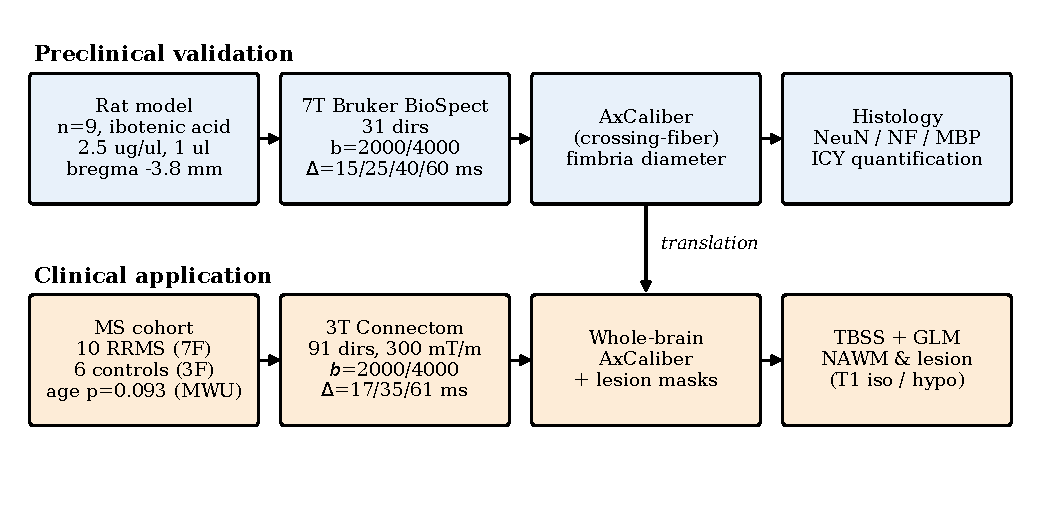
\includegraphics[width=0.95\textwidth]{figures/fig1_pipeline.pdf}
\caption{Translational experimental design. Top row: unilateral stereotaxic injection of ibotenic acid (2.5~\textmu g/\textmu l, 1~\textmu l) into the right dorsal hippocampus of $n=9$ rats (coordinates bregma $-3.8$~mm, sup-inf 3.0~mm, 2~mm from midline) produces Wallerian-like axonal damage in the fimbria; 14~days later, animals are scanned on a 7T Bruker BioSpect with a 31-direction diffusion protocol and then perfused for NeuN / neurofilament / MBP immunohistochemistry. Bottom row: an acquisition-matched AxCaliber protocol is deployed on a 3T Connectom scanner (300~mT/m, 64-channel array) in a cohort of 10 relapsing-remitting MS patients and 6 age-matched controls, followed by TBSS and GLM analysis of lesions and normal-appearing white matter.}
\label{fig:pipeline}
\end{figure}

% Figure 2 -- preclinical ANOVA and paired tests
\begin{figure}[htbp]
\centering
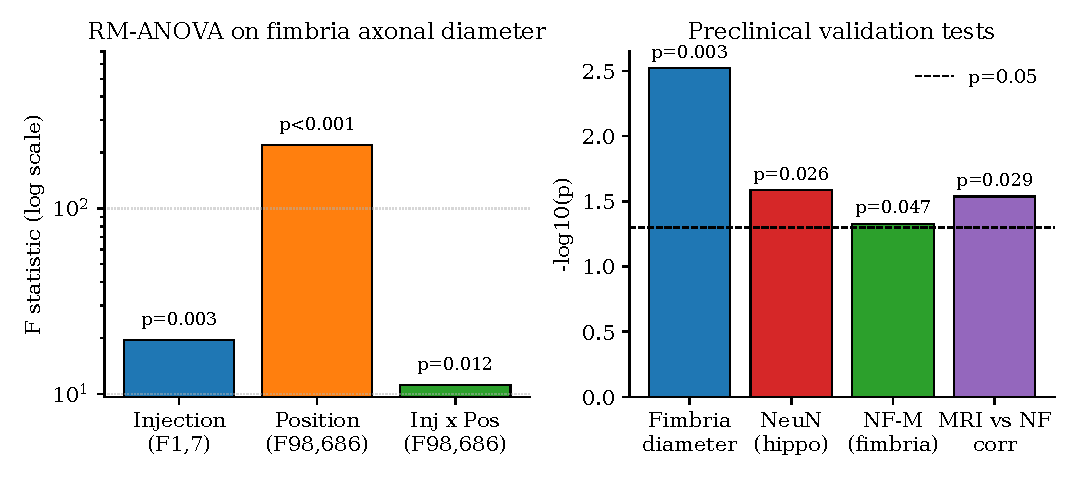
\includegraphics[width=0.95\textwidth]{figures/fig2_rat_stats.pdf}
\caption{Preclinical validation statistics. Left: repeated-measures ANOVA on the estimated axonal diameter along the antero-posterior fimbria (100 steps) reveals main effects of injection ($F_{1,7}=19.5$, $p=0.003$), tract position ($F_{98,686}=219.5$, $p<0.001$) and their interaction ($F_{98,686}=11.2$, $p=0.012$). Right: paired t-tests confirm axonal-diameter increase in the injected fimbria ($p=0.003$), neuronal loss in the hippocampus (NeuN, $p=0.026$) and increased neurofilament staining in the fimbria ($p=0.047$); MRI-derived axonal diameter correlates with neurofilament intensity across hemispheres ($r=0.54$, $p=0.029$). The dashed line marks $p=0.05$.}
\label{fig:ratstats}
\end{figure}

% Figure 3 -- MS clinical GLM
\begin{figure}[htbp]
\centering
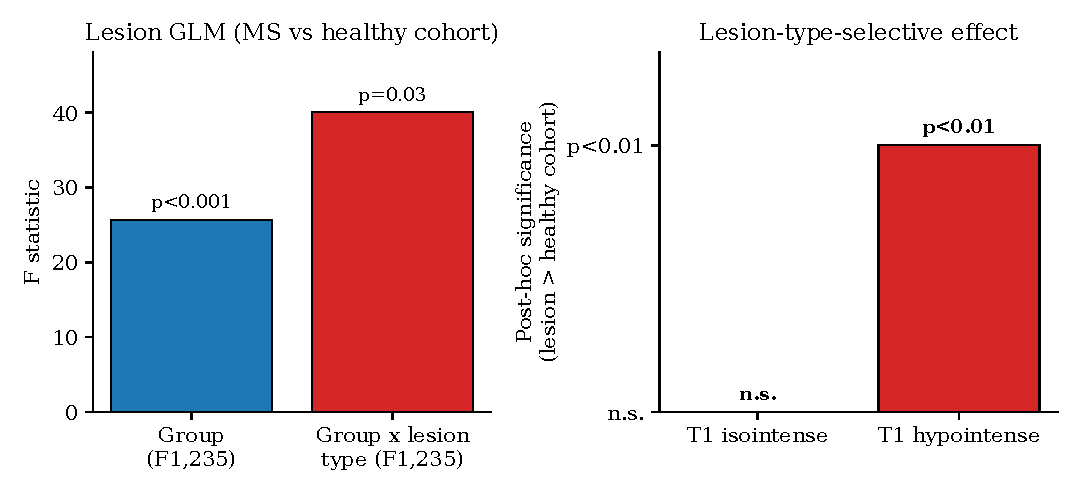
\includegraphics[width=0.95\textwidth]{figures/fig3_ms_glm.pdf}
\caption{Lesion-level GLM in MS patients vs the healthy cohort. Left: significant main effect of group ($F_{1,235}=25.7$, $p<0.001$) and group $\times$ lesion-type interaction ($F_{1,235}=40.1$, $p=0.03$). Right: post-hoc tests localise the effect to T1-hypointense lesions ($p<0.01$), with no significant difference in T1-isointense lesions. A one-sample $t$-test on the normalized index of asymmetry (NIA) further indicates that lesions have a significantly larger axonal diameter than contralateral normal-appearing tissue ($p<0.001$).}
\label{fig:msglm}
\end{figure}

% Figure 4 -- MRI/histology correlation summary
\begin{figure}[htbp]
\centering
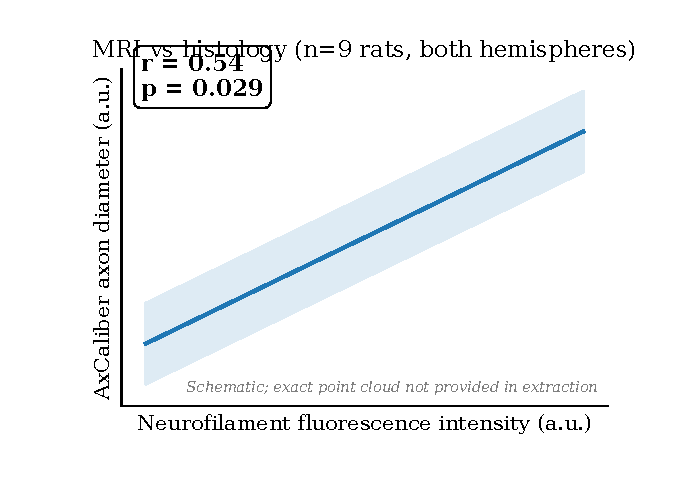
\includegraphics[width=0.6\textwidth]{figures/fig4_mri_histology.pdf}
\caption{Correlation between neurofilament fluorescence intensity (histology) and AxCaliber-derived mean axonal diameter (MRI) pooled across ibotenic-acid-injected and saline-injected fimbrias of $n=9$ rats: $r=0.54$, $p=0.029$. Shaded band is schematic; individual data points were not available in the extraction.}
\label{fig:mrihist}
\end{figure}

% Figure 5 -- TBSS placeholder
\begin{figure}[htbp]
\centering
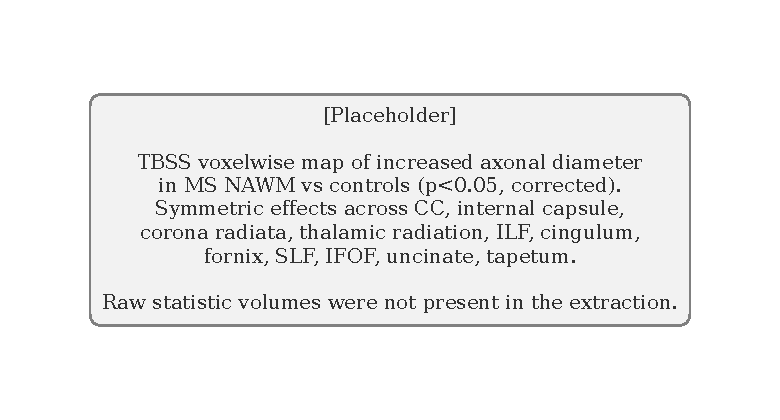
\includegraphics[width=0.7\textwidth]{figures/fig5_tbss_placeholder.pdf}
\caption{Whole-brain TBSS contrast (MS $>$ controls) for mean axonal diameter in the NAWM. Significantly increased axonal diameter was observed symmetrically in all major tracts examined, including the corpus callosum, internal capsule, corona radiata, thalamic radiation, inferior longitudinal fasciculus, cingulum, fornix, superior longitudinal fasciculus, inferior fronto-occipital fasciculus, uncinate fasciculus and tapetum ($p<0.05$, corrected). The reverse contrast was not significant. Placeholder panel: the underlying voxel-level statistic volumes were not available in the extraction.}
\label{fig:tbss}
\end{figure}
